\section{Introduction}

Big advantage of deep neural networks in general: They require a lot of data in order to generalize effectively.

Disadvantage of 3D convolutional neural networks: they treat the temporal and spatial domain equally.
Like a 3D object.

However: Temporal dimension is not equal to spatial dimension, i.e. adjacent frames correlate a lot by obbeying the laws of physics: Shown objects cannot instantaneously disappear and move with finite velocities.

Recently published charades datset. Very challenging!
Good classifiers on this dataset enable real-world applications for robotics.

\section{Related Work (Action Recognition)}

\subsection{Overview}

\subsection{C3D}
The work of \textcite{tran_learning_2015} provides a prominent example of a 3D convolutional archictecture, which does not require the explicit calculation of optical flow.
Optical flow has previously been incorporated in an additional temporal network stream by \textcite{simonyan_two-stream_2014}.
The network in \cite{tran_learning_2015} uses a volume of stacked video frames as input and therefore performs action recognition on raw RGB inputs only.
By training the network on the very large noisly labelled dataset Sports-1M \cite{karpathy_large-scale_2014}, the authors were able to train a generic spatio temporal feature extractor, which they call \textit{C3D}.
That is, the activations of the network's last fully connected layer can be used as a generic feature representation of the input.
An arbitrary classifier can then be trained on this input-representation to perform several differernt video-based vision tasks such as action recognition, scene classification or object detection.

The work of \textcite{karpathy_large-scale_2014} motivated the incorporation of 3D convolutions in \textit{C3D} by providing a comparative evaluation on different fusion strategies, i.e. on how to combine temporal and spatial information in different neural network architectures.
\textcite{tran_learning_2015} additionally conclude, the advantageous property of 3D convolutions, that temporal information is not immediately but gradualy condensed along the layer of a 3D CNN.

\begin{figure}[H]
    \centering
    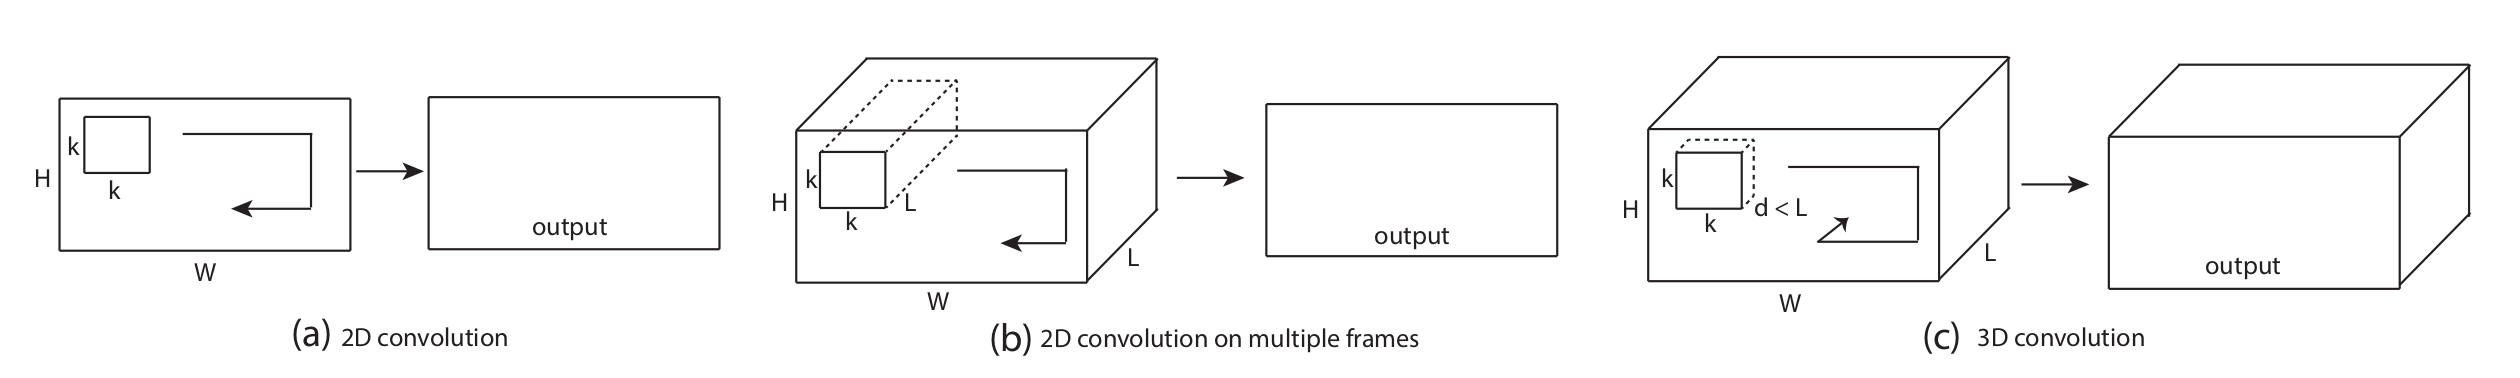
\includegraphics[width=\textwidth]{img_related/c3d_2dconv3dconv}
    \caption{Preservation of the temporal dimension by 3D convolutions: \textit{(a)} and \textit{(b)} 2D convolutions on a single or multiple frames results in a 2D feature map without temporal dimension. \textit{(c)} 3D convolutions on multiple input frames preserves the temporal dimension and results in a 3D feature map. \cite{tran_learning_2015}}
    \label{fig:c3d_2dconv3dconv}
\end{figure}

\textcite{tran_learning_2015} initially perform experiments on the smaller action recognition dataset UCF-101 \cite{soomro_ucf101:_2012}, to find the optimal size of kernels for the \textit{C3D} architecture. Results indicate, that kernels of size $3 \times 3 \times 3$ perform best.
The final architecture consists of 8 3D convolutional layers, 5 max-pooling layers, two fully-connected layers and a softmax output layer.
The architecture and layer sizes are illustrated in figure \ref{fig:c3d_architecture}.

\begin{figure}[H]
    \centering
    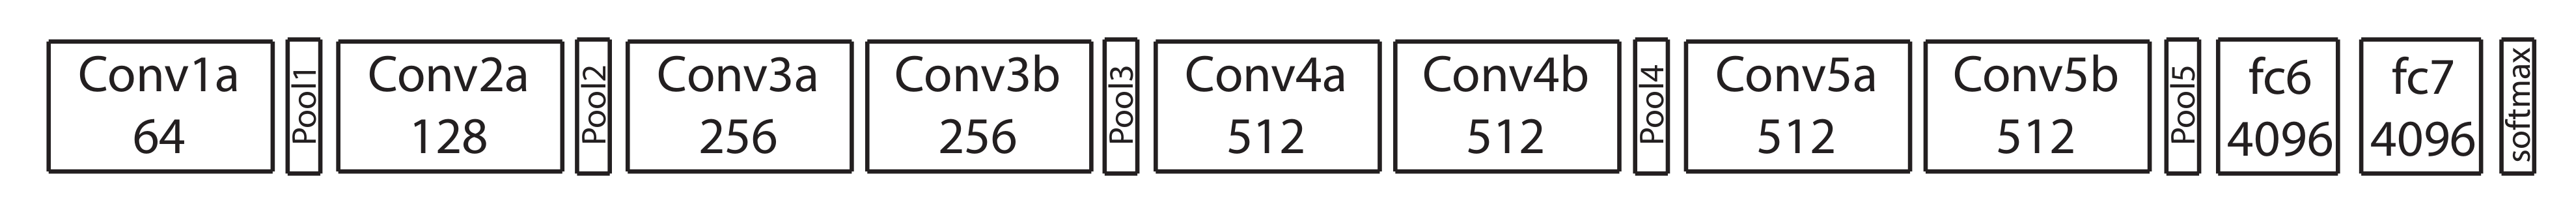
\includegraphics[width=\textwidth]{img_related/c3d_architecture}
    \caption{C3D architecture. Number of filters is given in each box. \cite{tran_learning_2015}}
    \label{fig:c3d_architecture}
\end{figure}

Final results when using a single \textit{C3D} network yield an accuracy of $82.3\%$ on UCF-101 \cite{soomro_ucf101:_2012}.
Note that these results were obtained from classifying the activations of the network's last fully-connected layer with an SVM.
The network was trained on the very large Sports-1M dataset \cite{karpathy_large-scale_2014} for this evaluation.
Only training the SVM on top of the networks activations uses the UCF-101 dataset.

Due to its competitive performance, the \textit{C3D} network is used as a prominent example of a 3D convolutional neural network using only raw RGB inputs.
\textcite{carreira_quo_2017} use it as main architecture to compare their own approach against.
Although the results of \textit{C3D} are competitive, the prototypical two-stream approach by \textcite{simonyan_two-stream_2014} outperforms \textit{C3D} by yielding $88.0\%$ accuracy on UCF-101.
Two-stream approaches are therefore considered the more successful architectures in action recognition \cite{wang_action_2015}, since they treat the spatial and temporal dimension differently.


\subsection{Temporal Order Verification}
\label{subsec:tov}

The work of \textcite{misra_shuffle_2016} is most related to ours.
The authors incorporate \textit{Temporal Coherency} between video frames to learn image representations, which are highly discriminative towards motion and therefore well suited for Action Recognition.
Our work is the logical continuation from learning these action representations with 2D CNNs as in \cite{misra_shuffle_2016} to 3D CNNs.

\textit{Temporal Coherency} describes an inherent relation between consecutive video frames.
More precisely, consecutive frames are semantically and dynamically correlated \cite{herath_going_2016}.
This means in terms of action recognition: Two consecutive frames are highly likely to present the same action and are limited by the laws of physics in the magnitute of change that can occur between them.

\textit{Temporal Coherency} can be used as a weak form of supervision in training deep networks, in contrast to strong supervision regular semantic labels.
\textcite{misra_shuffle_2016} propose an auxiliary quasi-unsupervised pre-training method which incorporates this \textit{Temporal Coherency} by first training a network on a binary classification task.
More precisely: The Network is presented with a sequence of input frames, which may have been randomly permuted, and has to determined if the sequence is in correct temporal order or not.
This pre-training task is called \textit{temporal order verification}.

This is, in the strictest sense, not an unsupervised training task, but since obtaining the label (\textit{correct temporal order} or \textit{incorrect temporal order}) is free, the authors attribute it as unsupervised \cite{misra_shuffle_2016}.
This has the advantage, that easily obtainable unlabelled data can be used for pre-training the network.

\textcite{misra_shuffle_2016} evaluate their approach by presenting three video frames to a triplet siamese CNN with 2D convolutions (see figure \ref{fig:shufflelearn_approach}).
Their results show, that using four or five frames did not result in an increase of performance.
Datasets utilized for training and evaluation are UCF-101 \cite{??} and HMDB-51 \cite{??}

\begin{figure}[H]
    \centering
    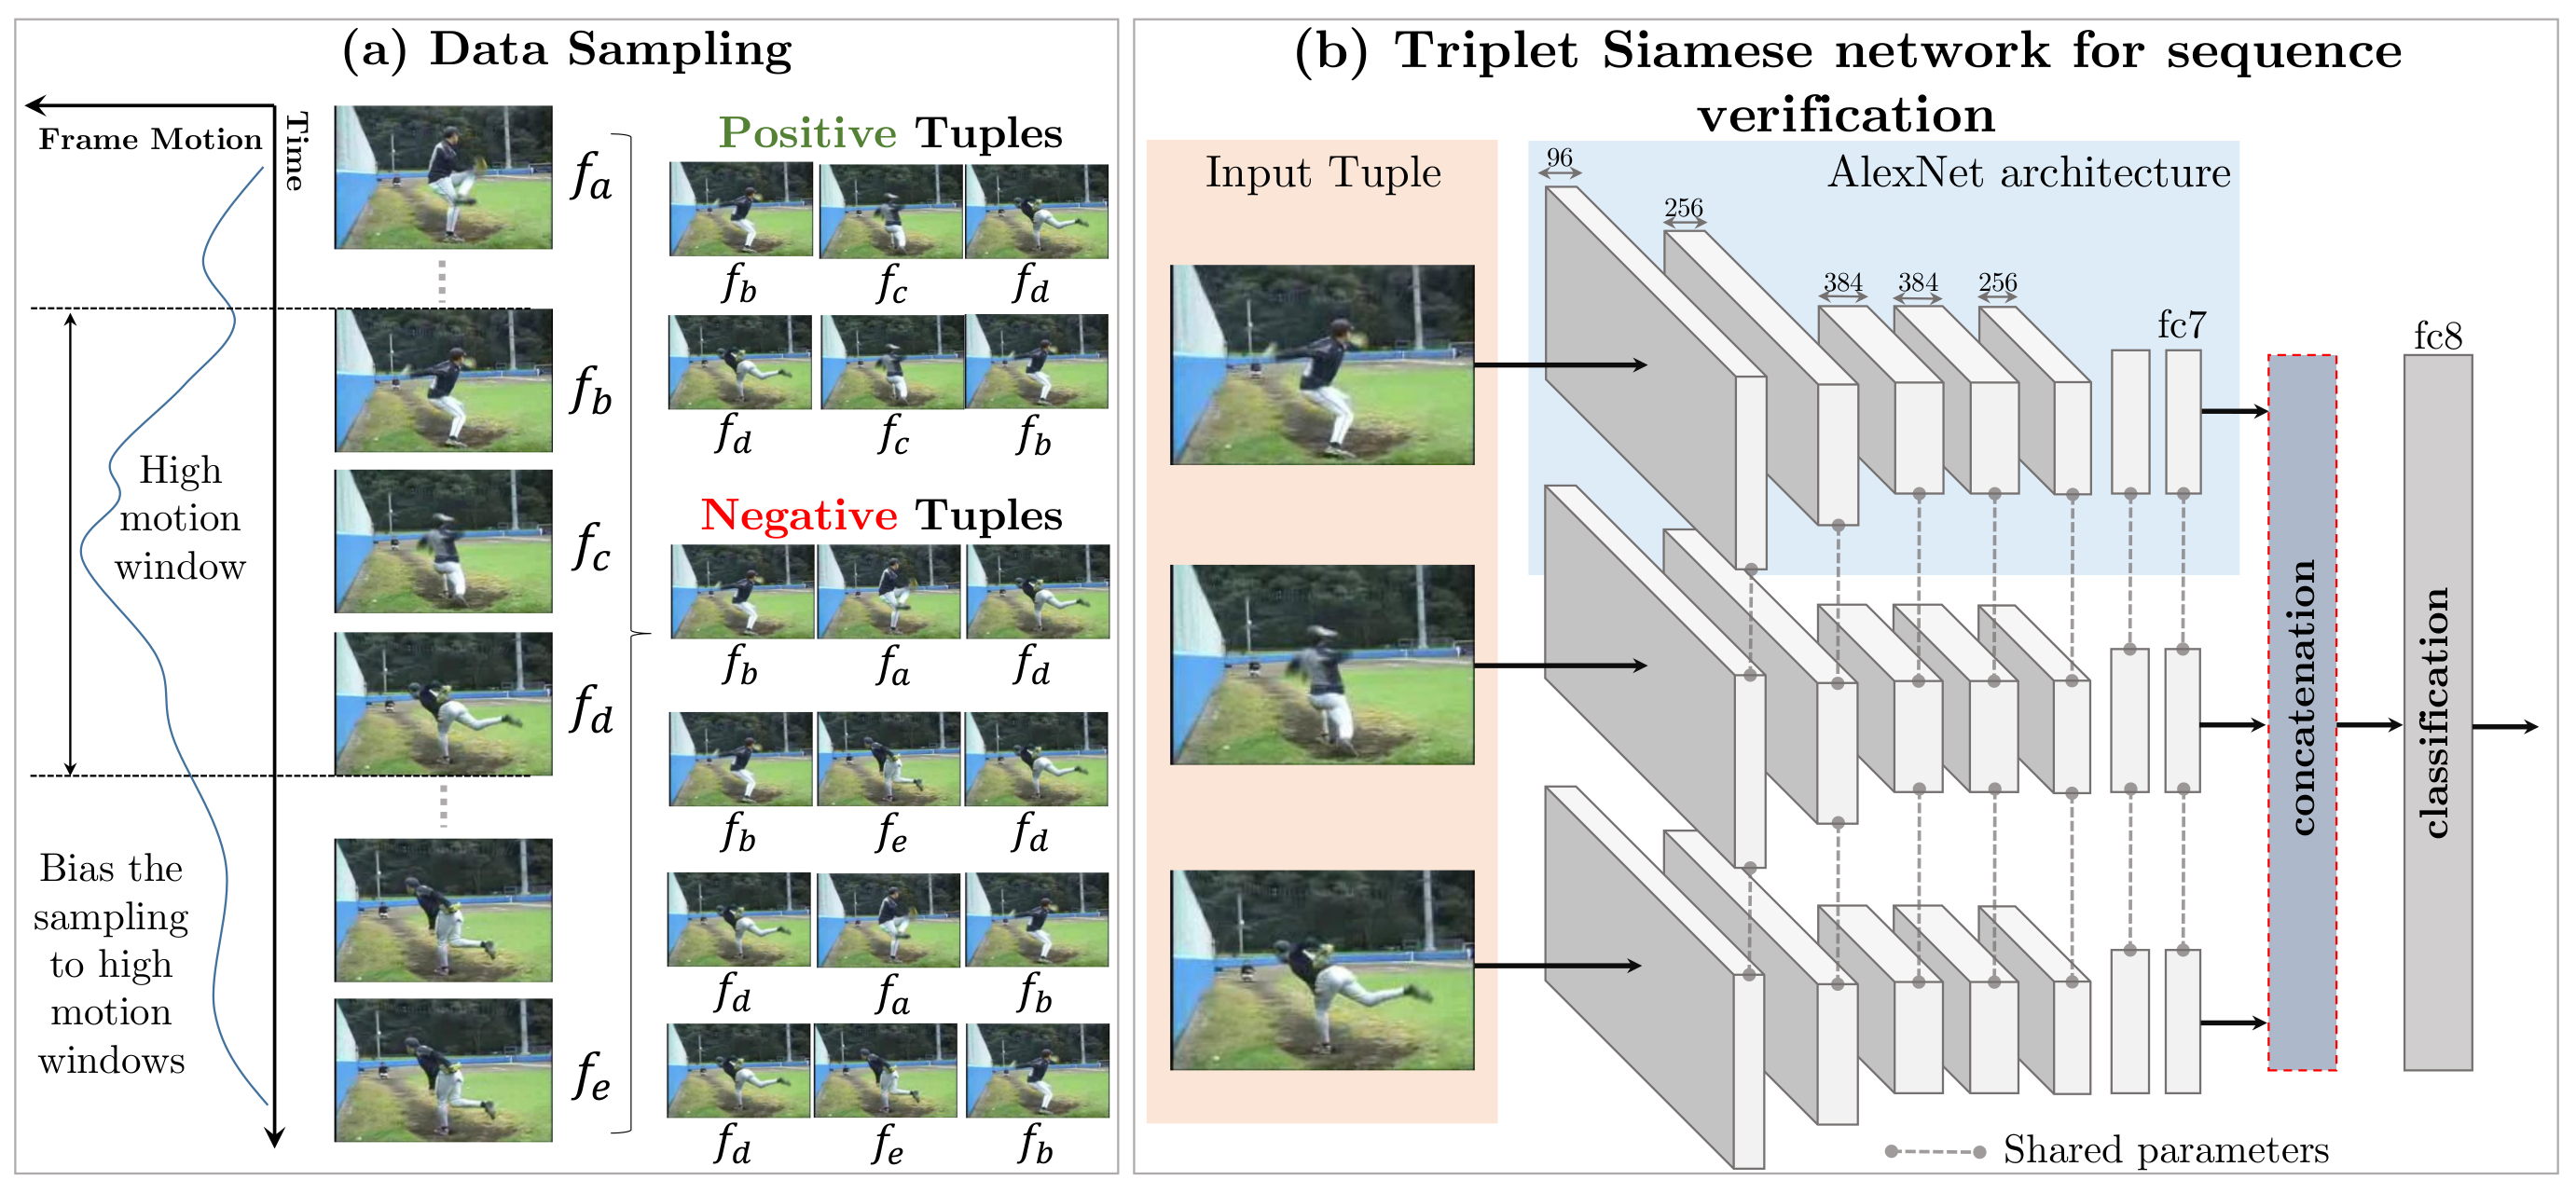
\includegraphics[width=\textwidth]{img_related/shufflelearn_approach}
    \caption{\textit{(Left)} Sampling of input sequences during temporal order verification. Sampling was biased towards regions with motion present in order to not obtain too similar frames. \textit{(Right)} Triplet siamese convolutional neural network, with shared weights. \cite{misra_shuffle_2016}}
    \label{fig:shufflelearn_approach}
\end{figure}

The authors use optical flow between two frames \cite{farneback_two-frame_2003} to identify a high motion window in the input video and construct positive examples (\textit{correct temporal order}) and negative examples (\textit{incorrect temporal order}) from the frames contained in it.
This ensures a certain magnitude of motion between the sampled frames and results in frame tuples, which are clearly distinguishable when permuted.

More precisely: Five frames $\{f_a, f_b, f_c, f_d, f_e\}$ are sampled from an input video, with $a < b < c < d < e$.
Out of these $f_a, f_b, f_c$ need to lie in the high motion window.
$f_b$ and $f_d$ are taken as start and end of the input sequence.
To construct a negative example (\textit{wrong temporal order}), $f_e$ or $f_a$ are inserted as middle frame to complete the input sequence.
The authors note, that it is vital to keep $f_b$ and $f_d$ as beginning and end of the input, i.e. the correct frames of the middle triple.
A mere inversion, i.e. $f_d, f_c, f_b$ is used as positive examples.

The incorporated network is available in the Caffe-Framework \cite{jia_caffe:_2014-1} and is called CaffeNet, an adapted version of the AlexNet model \cite{krizhevsky_imagenet_2012-1}.
The CNN model is arranged as a siamese triplet, with weight sharing.
That is: three identical copies of the network model each process one input frame, the results activations of the fully-connected layer are concatenated and then classified by an additional fully connected layer.
The individual network models share weights, i.e. each of them receive the same weight updates.

Results are obtained by training the composite model on UCF-101 and HMDB-51.
The model is either trained from scratch (weights are randomly initialized), pre-trained with \textit{temporal order verification} (weights are initialized from a pre-trained model) or pre-trained on UCF-101 for the evaluation on HMDB51.

\begin{table}[H]
    \centering
    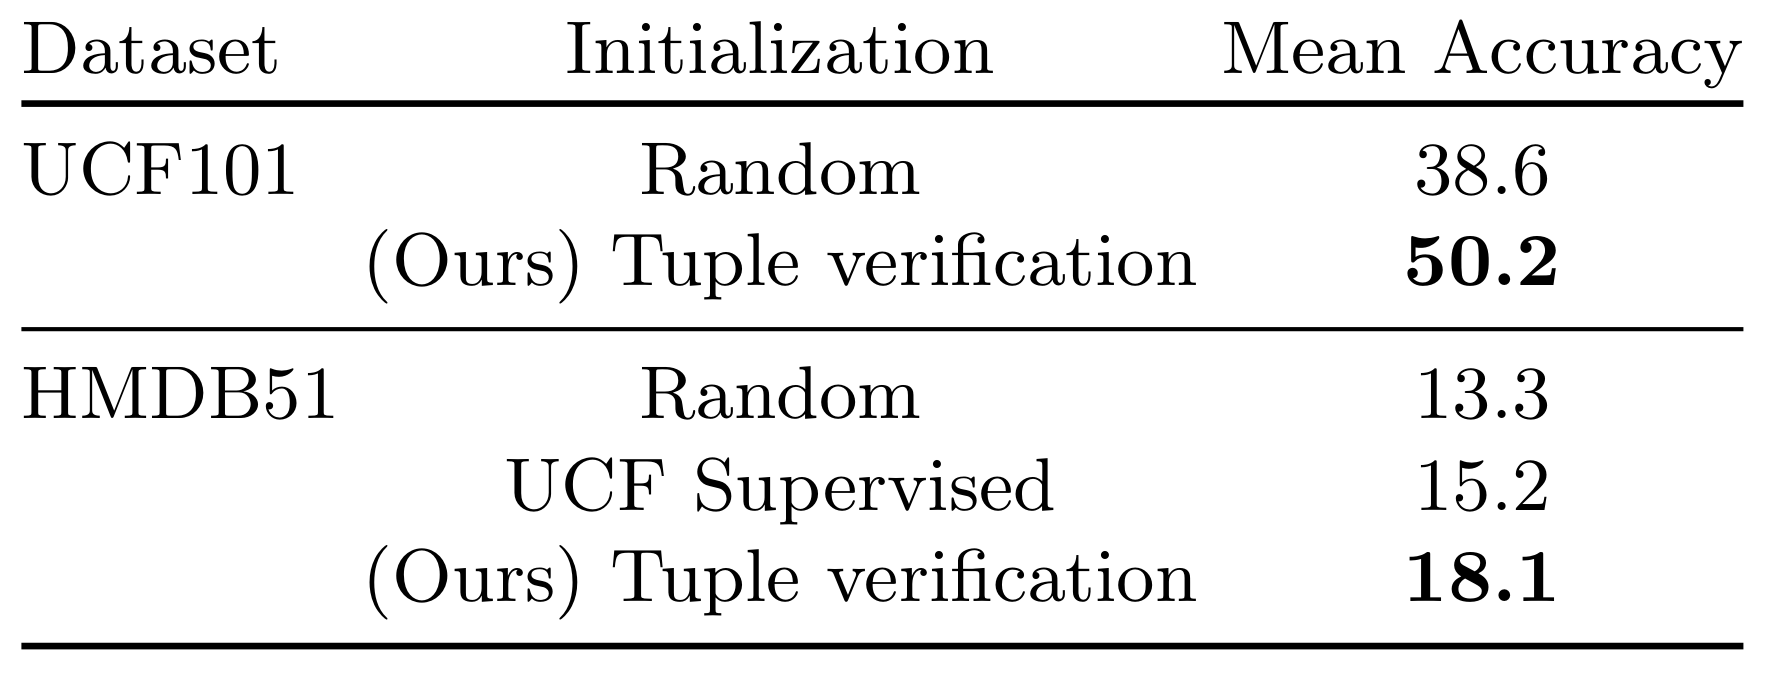
\includegraphics[width=0.6\textwidth]{img_related/shufflelearn_results}
    \caption{Perfomance gain in mean accuracy when incorporating temporal order verification as weight-initialization method on UCF-101 and HMDB-51 \cite{misra_shuffle_2016}}
    \label{tab:shufflelearn_results}
\end{table}

Table \ref{tab:shufflelearn_results} shows the increase in final performance after fine-tuning the model on either UCF-101 or HMDB-51.
The increase in performance of $+11.6\%$ is most prominent on UCF-101.
On HMDB-51 initializing the model using \textit{temporal order verification} achieves an increase in accuracy of $+4.8\%$, which is smaller than on UCF-101 but still significant.
Notably initialization from \textit{temporal order verification} outperforms initiliazing the network from regular pre-training on labeled data.
\bigskip

\textbf{Implementational details:}\\
\begin{itemize}
    \item The authors did not use any additional unlabeled data for pre-training, but sample around $900$k triples for \textit{temporal order verification} from the labeled datasets itself.
    \item Weights are randomly initialized for the \textit{temporal order verification} pre-training. 
    \item Pre-training is conducted for $100$k iterations with a fixed learning rate of $10^{-3}$ and a batch-size of 128 tuples (This results in around $14$ epochs in total for a pre-training set of $900$k triples).
    \item Best results were obtained with $25\%$ positive and $75\%$ negative triples.
    \item Batch normalization \cite{ioffe_batch_2017} is used during training.
    \item A single CaffeNet model is then initialized from the weights obtained from pre-training the siamese triplet. It is trained for $20$k iterations with a batch size of $256$ frames on UCF-101 and HMDB-51.
    \item The learning rate used for fine-tuning the model $10^{-2}$, which is decayed to $10^{-3}$ after $14$k iterations.
    \item Evaluation results are obtained from averaging random crops and flips from each test-video. First $25$ frames are uniformly sampled per video, $5$ input-sized regions are cropped out and flipped. This results in a total of $250$ inputs for averaging per video ($25$ frames $\times$ $5$ crops $\times$ $2$ flips).
\end{itemize}
